\documentclass[a4paper,12pt]{article}
\usepackage{hyperref}
\usepackage{times}
\usepackage{comment}
\usepackage{titlesec}
\usepackage[pdftex]{graphicx}

\usepackage{geometry}
\geometry{lmargin=1.5cm,rmargin=1.5cm,height=25cm}
\renewcommand{\thesubsection}{\Roman{subsection}}

\begin{document}

\title{The Anastasis: an Easter icon at the Wignacourt Museum, Rabat, Malta.}

\author{Joanna Lace} 

\date{Easter 2009} 

\maketitle 

\begin{figure}[htbp]
\centering
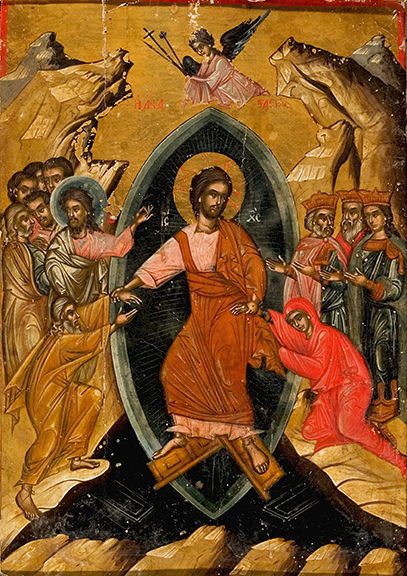
\includegraphics[width=12cm]{anastasis1.png}
\caption 
{\it The Anastasis.   Tempera on panel, 41 cm x 28 cm.  Wignacourt Museum,
Rabat, Malta.} 
\end{figure}
``The feast of Easter'', says St.~Gregory the Theologian in an Easter
sermon, ``is for us the feast of feasts and the celebration of
celebrations, it excels all other festivals, as the sun excels the
stars..''.  This annual celebration of the Resurrection of Christ is
expressed visually by orthodox Christians by means of the icon known
as the ‘Anastasis’-–-the Greek word for resurrection---the title in
this example being inscribed in red lettering above the central figure
of Christ that dominates the scene.  Christ is also identified, the
letters IC XC being the first and last letters of the two Greek words
for the name Jesus Christ; a bar above the letters indicating a sacred
name.  It is an icon that can bring new insights to those of us more
conversant with the visual repertoire of western Christianity.

As a prefix to its interpretation, a few words concerning western
traditions are in order, in that western artists depicted Christ’s
resurrection rather differently.  They show him literally rising
triumphant from an empty tomb, a scene that might be followed by a
version of the anastasis composition renamed as the Descent of Christ.
Furthermore, the newly acquired title becomes qualified in the west
according to Christ’s destination: this may be given as ‘Hell’ (and
hence the familiar ‘Harrowing of Hell’), ‘Hades’, or ‘Limbo’---often
regardless of the details of the composition, which may or may not
include the figure of Hades and dramatic struggles with Satan.
Whether arbitrary or not, these different destinations pose
theological questions that will not be dealt with in this analysis,
which will concentrate upon the uncovering and evaluating of the
message transmitted visually by a classical Easter icon.  It would
also be true to say that no viewer with a Christian background.would
have much trouble understanding its message in general terms of
Christ’s saving of threatened humanity.  Resplendent, calm, and
surrounded by an eager crowd of onlookers---some crowned, one a
saint---he draws towards himself a man and a woman from the edge of a
dark pit.  It is when details of the composition are analysed that the
full impact of the message can be understood: it is one in which the
historical (as narrated in the Gospels) is united with the cosmic, so
as to be seen by the contemplative viewer as one seamless whole.

\subsubsection*{THE MESSAGE CONVEYED}

\begin{figure}[htbp]
\centering
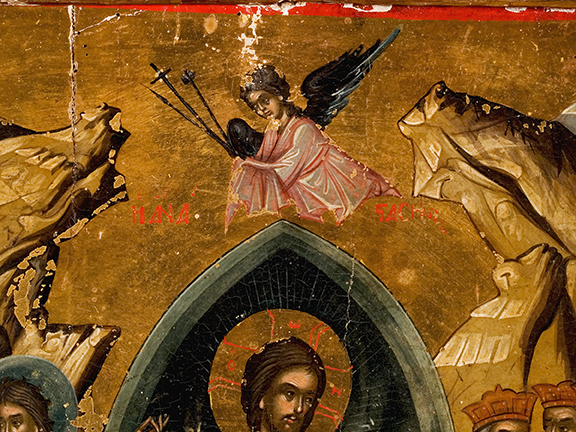
\includegraphics[width=8cm]{anastasis2.png}
\caption 
{\it The Anastasis (detail).} 
\end{figure}
The subject is introduced by an angel seen hovering at the icon’s
upper edge in a narrow opening between two rugged mountain peaks.
These peaks curve inwards towards each other as if, but for the
angel’s presence, they would enclose the central scene.  The angel
carries aloft three symbols known as the Instruments of Passion: the
spear with which a soldier had pierced Christ’s side, the Cross of his
crucifixion, and the reed holding a sponge filled with the vinegar
that was given Him to drink.  These indicate that the crucifixion has
taken place: it is that moment when ``the earth shook and rocks were
split'' (Matthew 27:51), an event of pain and cruelty that appears to
be echoed in the terrifying landscape that encroaches on either side
The angel bends over the central figure of Christ: a figure shown not
as a human body after suffering the torments of the cross, but erect,
transfigured, clothed in bright garments.  His halo is inscribed with
the Greek letters ``O W N'' (``The One Who Is''): the name of God that
was given by God himself to Moses (Exodus 3:14).

Christ is enclosed within a mandorla, which sweeps down through the
rocky ground to pierce the utter darkness of a cave-–-the underworld.
His feet are planted upon its broken gates, and as he stands astride
the opening, eager hands from the crowd on either side reach through
the mandorla towards him.

Much of the meaning of the Anastasis icon is revealed by the various
crossings of the boundary of this mandorla, which was an ancient
symbol now used by Christians to indicate the line of separation of
the earth from the unknown regions beyond.  Marking this division were
the heavens, usually shown, as here, by concentric bands in shades of
blue that darken towards the boundary.  The boundary is crossed in
opposite directions: inwards by those reaching towards Christ; and
outwards by Christ himself, who grasps with either hand the leading
figure of the group on each side. In addition, from his person bright
rays shine out in all directions to pierce the heavens.  They are a
reminder that though the living Christ within the mandorla is now
outside earthly time and space and beyond full human understanding,
intimations of His divinity, majesty and mystery are continually being
sent out to reach humankind.

What we see in this Easter icon is plainly the effect of a miraculous
event, rather than the event itself.  Christ’s resurrection was not
witnessed by humans, and is not described in the Gospels; and Orthodox
theologians deemed that, as a simple act of God, it could not possibly
be expressed visually: only the effect of God’s action upon humankind
could be represented.  The effect is conveyed by visual metaphor---the
‘making of the invisible visible’.  Visual metaphor indeed is an
essential part of devotion to Christ for the orthodox Christian, for
whom the visual combines with theology, prayer, and the liturgy to
create one seamless whole.  In this way, the illustration of a
biblical figure may incorporate details that for the orthodox bring to
mind the words of a well-known theologian or preacher of recent date.

Turning now from Christ to the groups on either side: from certain
figures we learn that Christ is visiting those who have died before
his crucifixion.  Collectively they are known as ‘the righteous’, or
‘the just’: those who on earth have striven to know God, and who may
have lived saintly lives.  They are not suffering, but through the
centuries, due to man’s heritage of original sin, they have been
imprisoned in the underworld, not free to live a full life with God.
Amongst those on Christ’s right side the most prominent is St.~John
the Baptist, who wears the antique mantle of a prophet.  The first two
letters of the Greek form of his name are just visible, inscribed in
red beside his halo---the latter indicating his death as a martyr.  He
is known as St.~John the Forerunner ({\it podromos}), and the
declamatory aspect of his mission is emphasized visually by a broad
sweep of one arm so far across the boundary of the mandorla that his
hand reaches close to the head of Christ; whilst his other hand is
veiled in expression of his devotion.  At the same time, St.~John’s
head turns away from the mandorla to face the animated group assembled
behind him: his stance thus combines the depth of his own faith in
Christ with his call to preach Christ’s word to others as described in
the gospels.

On Christ’s left, the crowned figures in imperial dress are righteous
rulers of the Old Testament.  Foremost is King David, celebrated as
the greatest King of Israel: a many-sided monarch, venerated as author
of the Psalms, for his music, and notably for his humility and
penitence for the sins he committed.  Through the heroism of his
victory over Goliath he was considered to be a prefiguration of
Christ’s victory over Satan.  Standing next to him and shown, as
usually, young and beardless, is his son and successor, King Solomon,
considered to be the embodiment of all wisdom and righteousness,
author by ancient tradition of the Old Testament Books of Proverbs,
Ecclesiastes, and the Song of Songs, and the builder of the Holy
Temple in Jerusalem for the Ark of the Covenant.  Father and son both
extend open hands towards Christ in the conventional gesture of
acceptance.  The right hand of King David, as the prefiguration of
Christ, has reached across the border of Christ’s mandorla, and at the
same time he turns his head in order to look directly at his attentive
son, thus expressing the solidarity of an enlightened ruling dynasty.

At the head of these two groups of the righteous are the figures of
Adam to our left and Eve to our right, representing the rest of
mankind going further back in time to the early days of Creation.  The
particular form they are given here may be unfamiliar to Western eyes,
more used to a young and graceful man and woman walking together in
the Garden of Eden.  Here humanity is shown as it had become following
their disobedience, recriminations, and final expulsion by God from
the Garden.  Adam has reached old age, after years of toil, his
gesture illustrating words from the Psalms of David: ``Hear the voice
of my supplication ... as I lift up my hands towards thy most holy
sanctuary.'', and ``I will extol thee, O Lord, for thou has drawn me
up, and has not let my foes rejoice over me.'' (Psalm 28/27).

Eve, the ‘mother of mankind’, is almost completely enveloped in her
maphorion, the traditional garment worn by holy women, and as usual
for Eve, shown in red.  It is by means of this garment in fact that
the veiling of her hands-–-well-attested as expressive of awe and
respect---has been extended visually to cover the whole of her person,
revealing only her face, downcast, and the hand that Christ himself
has uncovered.  Its outline emphasises her gesture of deep reverence,
known by the Greek word {\it proskynesis} (in Latin, {\it adoratio}),
and which in Eve’s case here is the full prostration, indicating an
intensity of prayer and entreaty---the gesture used to illustrate the
words of the repentant David when rebuked by the Prophet Nathan: ``I
have sinned against the Lord'' (2 Samuel 12:13).

Christ’s gesture as he takes hold of repentant mankind, Adam with one
hand and Eve with the other, is depicted in a specific manner, with an
interesting history.  He does not simply take an outstretched hand in
his, but in each case his fingers grasp firmly around the wrist.  In
ancient Greece and Rome this gesture symbolised legal possession: a
bride, for instance, was ‘in the hand’ of her parent (father or
mother), who on the wedding day would accordingly grasp the daughter’s
wrist and place her hand into that of her husband..  Again, in
well-mannered society it conveyed a sense of leading, guiding and
protection, as when a host would politely guide his guest to the
appointed place in his house or at table.  It became part of Christian
iconography, and in the context of the anastasis---the moment of
mankind’s redemption through the sacrifice of His Son---it signals
quite simply the return to God of God’s own.

At this point the individual images surrounding Christ combine to give
the full meaning of the anastasis message: that from the moment of
Christ’s sacrifice all humanity has been freed from sin, all are born
anew, and all are now brought by Christ to live in God’s timeless
world.  It might be said that the composition as a whole invites
comparison with a text from the New Testament: the parable of the
prodigal son, one of the parables told by Christ himself during his
life on earth, and based for his audience on earthly, contemporary
life (Luke 15:11-32). In the icon a newly resplendent Christ within a
mandorla becomes himself the forgiving welcoming ‘father’ of the
parable, whose ‘home’ is now visualised in eternal, cosmic terms.

The event of the Anastasis is commemorated on Great Saturday (Easter
Saturday), and its associated icon is called the ‘Easter’ icon as a
prefiguration of the coming celebration.  It is integral to the
sequence of icons that illustrates the cycle of Great Feasts
throughout the year, and that embellishes the church’s iconostasis,
the screen marking the boundary between the human world and the
spiritual world of the sanctuary.  By the presence of the icons, the
two worlds are reconciled and united.  It seems that the Easter icon,
in particular, demonstrates this union: it shows events that have
taken place in the earthly world of time and space, that through
Christ’s sacrifice have been transposed and are part of God’s
spiritual and timeless reality.

\subsubsection*{FURTHER STUDY}

The fact that the Wignacourt icon is inscribed in Greek does not
indicate that it was painted in Greece, or in a Greek-speaking
province, Greek being the ecclesiastical language, in much the same
way as Latin in the West Provenance will not be easy to research.
Over the centuries, at different times in different regions of the
orthodox world, the basic composition has undergone numerous changes
in style: the figure of Christ, for example, has varied in degree from
the graceful and flamboyant, to a firmer, even stern stance.  Again,
the position of Eve varies: during earlier centuries she is normally
shown awaiting her turn immediately behind Adam.  It seems that our
balanced composition, where Christ takes one in either hand, became
more common during the fourteenth century.  It was chosen early that
century, albeit in a contrasting style, for the fresco of the
anastasis decorating the apse of the parekklesion in the former Chora
Monastery, now the Karije Camii mosque, in Istanbul, ---and chosen, as
often, for a funerary chapel.  Notable also over time are variations
in the Old Testament figures chosen for inclusion amongst the
righteous: their comings and goings have been analysed by
A~D.~Kartsonis in her useful publication {\it Anastasis: The Making of
  an Image} (Princeton, 1986).

Whilst the Anastasis icon itself is a treasure that merits further
study, the interpretation of its Easter message reveals to us, perhaps
with a new clarity, some of the deep meaning given by orthodox
Christians to the ``feast of feasts''.
\end{document}
